\chapter{Fundamentação Teórica}

Neste capítulo serão apresentadas as bases teóricas que permeiam o escopo do presente trabalho.
Partindo do entendimento sobre o conceito de arquitetura de software e como ela reflete nos
sistemas. Em seguida, abordando estilos de arquitetura de software pertinentes para o contexto
estudado. As seções estão dispostas em:

  \begin{enumerate}
    \item \textbf{Arquitetura de software:} definição do termo arquitetura dentro da área de
        software e suas características.
    \item \textbf{Sistemas monolíticos:} descrição, vantagens e desvantagens da arquitetura monolítica.
    \item \textbf{Microsserviços:} descrição, vantagens e desvantagens da arquitetura de
        microsserviços.
  \end{enumerate}

\section{Arquitetura de Software}

\begin{quotation}{Bass2015:SoftwareArchitetureInPratice}{transleted=true}
Software systems are constructed to satisfy organizations' business goals. The architecture is a bridge between those (often abstract) business goals and the final (concrete) resulting system. While the path from abstract goals to concrete systems can be complex, the good news is that software architecture can be designed, analyzed, documented, and implemented using know techniques that will support the achievement of these business and mission goals. The complexity can be tamed, made tractable.
\end{quotation}

Como retratado na citação acima, arquitetura de software representa a ponte entre os sistemas
construídos e os objetivos de cada organização. A publicação \textit{What is your definition of
software architecture?} do \textit{Software Engineering Institute} da \textit{Carnegie Mellon
University} \cite{SEI2017:WhatIsYourSoftwareArchitectureDefinition} apresenta uma variedade de diferentes
conceitos a respeito de arquitetura de software abordados pela bibliografia, exemplificando a
dificuldade existente em compreender o conceito de arquitetura dentro da área de \gls{TI}.

Segundo \citeonline{Vogel2011:SoftwareArchiteture} arquitetura é um aspecto implícito com o qual os desenvolvedores são confrontados
diariamente e que não pode ser ignorado ou eliminado, ainda que eles nem sempre tenham consciência
sobre a sua constante presença.

\citeonline{Bass2015:SoftwareArchitetureInPratice} traz a seguinte definição a respeito de
arquitetura de software:

\begin{quotation}{Bass2015:SoftwareArchitetureInPratice}{transleted=true}
The software architecture of a system is the set of structures needed to
reason about the system, which comprise software elements, relations
among them, and properties of both.
\end{quotation}

Com base nessa abordagem, os autores defendem que os sistemas de software são compostos por diversas
estruturas e elementos, por como essas estruturas se relacionam entre si e pelas propriedades que os
caracterizam. Assim, a arquitetura se torna uma abstração do sistema, destacando aspectos desejados
do mesmo e omitindo outros aspectos, com o intuito de minimizar a complexidade com a qual o compreendemos.

A \autoref{fig:ArchitectureDefinition} apresenta uma segunda visão abordada por
\citeonline{Richards2020:FundamentalsOfSoftwareArchitecture} a respeito de arquitetura.
Nessa abordagem eles defendem quatro dimensões as quais definem o que é arquitetura de software. A primeira
dimensão consiste nas estruturas: serviços, camadas e módulos são exemplos de conceitos abarcados
por esse ponto, todavia, para eles descrever a arquitetura por meio de estruturas não é suficiente para contemplar
todo o escopo acerca de arquitetura de software. Diante desta problemática, eles introduzem os
conceitos de características, decisão e princípios de design referentes a arquitetura. 

\begin{figure}[h]
  \centering
  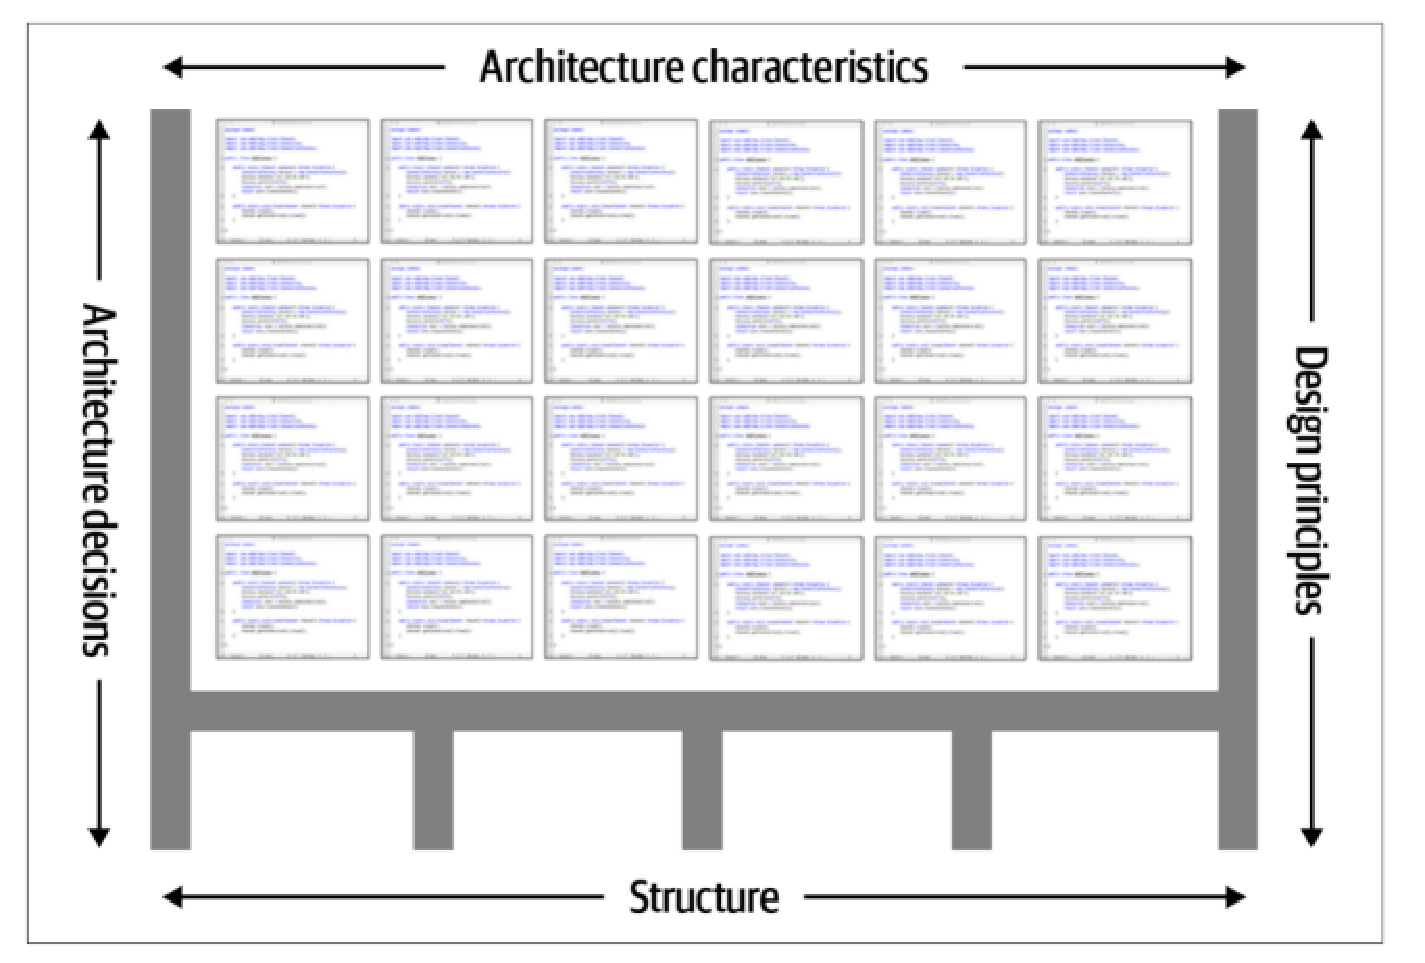
\includegraphics[keepaspectratio=true,scale=0.6]{figuras/richardsAndFord-architectureDefinition.eps}
  \caption{Elementos que compõem a arquitetura de um software\label{fig:ArchitectureDefinition} \source{Richards2020:FundamentalsOfSoftwareArchitecture}}
\end{figure}

As características da arquitetura, por sua vez, referem-se aos critérios de sucesso do sistema,
trazendo pontos como disponibilidade, confiabilidade, segurança, etc., os quais são anteriores e
independentes ao conhecimento acerca das funcionalidades que o software implementará.

O terceiro aspecto apresentado pelos autores consiste nas decisões de arquitetura responsáveis por definir
as regras sob as quais o sistema deve ser construído. Isto diz ao time de desenvolvimento o que ele
pode ou não fazer. A exemplo, em uma arquitetura \gls{MVC}\footnote{\textit{Model-View-Controller} (MVC)
consiste em um estilo arquitetural adotado por várias aplicações. A \textit{Model} representa a
camada de dados, a \textit{View} a camada de apresentação e a \textit{Controller} é a camada de
lógica \cite{mcgovern2004practical}.}, a \textit{View} é
impossibilitada de consumir dados da \textit{Model}, e cabe aos desenvolvedores garantir que isso
seja respeitado.

Por fim, a última dimensão refere-se aos princípios de design. Estes consistem em um guia pelo o qual
os desenvolvedores podem se orientar quando for necessário tomar alguma decisão. Diferentemente das
decisões de arquitetura que devem ser sempre seguidas afim de  garantir as características desejadas
para a arquitetura, os princípios trazem maior flexibilidade e autonomia para o desenvolvedor, podendo
este analisar o contexto do problema em mãos e decidir se seguir os princípios é a melhor abordagem
para a funcionalidade desenvolvida, ou se deve seguir por um caminho diferente o qual ele julgue que
os ganhos são maiores para a aplicação.

\subsection{Leis da Arquitetura de Software}

\begin{quotation}{Richards2020:FundamentalsOfSoftwareArchitecture}{transleted=true}
  \begin{description}
    \item [Tudo em arquitetura de software é um \textit{trade-off}.] Primeira Lei da Arquitetura de
        Software
    \item [\textit{Por que} é mais importantes do que \textit{como}.] Segunda Lei da Arquitetura de Software
  \end{description}\footnote{Texto original: \textit{Everything in software architecture is a trade-off. First Law
    of Software Architecture. Why is more important than how. Second Law of Software Architecture.}}
\end{quotation}

As leis acima foram apresentadas recentemente por \citeonline{Richards2020:FundamentalsOfSoftwareArchitecture}
no livro \textit{Fundamentals of Software Architecture: An Engineering Approach} e trazem consigo
perspectivas importantes para compreender o que é arquitetura de software dentro do dia a dia dos
engenheiros de software e como os mesmos devem lhe dar com ela.

A Primeira Lei da Arquitetura de Software descreve a realidade do arquiteto de
software, o qual precisa lidar constantemente com conflitos de escolha. O papel do arquiteto está
intrinsecamente ligado a análise da situação e a tomada de decisão sobre qual caminho seguir. Para
tal, é necessário que o mesmo esteja alinhado com uma série de fatores, como práticas de engenharia,
\textit{DevOps}\footnote{\textit{DevOps} é um movimento cultural que altera como indivíduos pensam
sobre o seu trabalho, dando suporte a processos que aceleram a entrega de valor pelas empresas ao
desenvolverem práticas sustentáveis de trabalho \cite{davis2016effective}.}, processos, negócio, etc
\cite{Richards2020:FundamentalsOfSoftwareArchitecture}.

A segunda lei traz uma perspectiva que por diversas vezes é ignorada, na qual tendemos a olhar para
a topologia dos sistemas, observando suas estruturas e como estas se relacionam, e não damos a devida
atenção ao porquê das decisões arquiteturais tomadas \cite{Richards2020:FundamentalsOfSoftwareArchitecture}.

Nesse sentindo, o ponto defendido pelos autores busca olhar o por quê certas decisões são
tomadas mediante os \textit{trade-offs} enfrentados.

\section{Sistemas monolíticos}
\label{monolithics}

A visão inicial a respeito da Arquitetura Monolítica refere-se a um padrão de desenvolvimento
de software no qual um aplicativo é criado com uma única base de código, um único sistema de compilação,
um único binário executável e vários módulos para recursos técnicos ou de negócios. Seus componentes
trabalham compartilhando o mesmo espaço de memória e recursos formando uma unidade de
código coesa \cite{NatalliaSakovich}.

\citeonline{newman2019monolith} expande um pouco dessa visão, saindo da ideia de uma única base
de código coesa e adotando a perspectiva de uma única unidade de \textit{deploy}. Essa abordagem
permite a ele distinguir os seguintes tipos de monolíticos:

\begin{description}
    \item [Monolítico com um único processo] é o tipo mais comum de monolíticos e refere-se
        fundamentalmente a existência de um único processo executando toda a base de código. Vale
        ressaltar que dentro desta classificação exite ainda um subconjunto de monolíticos
        modulares nos quais têm se cada módulo trabalhando de forma independente um do outro, mas
        ainda com a necessidade de implantar uma única unidade de código.

    \item [Monolítico distribuído] são sistemas compostos por múltiplos serviços mas que precisam
        ser implantados juntos. Nas palavras de \citeonline{newman2019monolith}:

        \begin{quotation}{newman2019monolith}{transleted=true}
            Um monolítico distribuído pode muito bem atender a definição de uma
            \gls{SOA}\footnote{A Arquitetura orientada a serviço - SOA é uma abordagem arquitetural na qual
            vários serviços trabalham juntos para entregar um conjunto de funcionalidades.
            \cite{Newman2015}}, mas muitas vezes falha em cumprir as promessas do padrão.
            \footnote{Texto original: \textit{A distributed monolithic may well meet the definition of a
            service oriented-architecture, but all too often fails to deliver on the promises of SOA.}}
        \end{quotation}
    \item [Sistemas caixa preta de terceiros] também são abordados por \citeonline{newman2019monolith}
        como sendo monolíticos, uma vez que não é possível decompor os esforços referente a uma
        migração.
\end{description}

\subsection{Estrutura de um monolítico}

A arquitetura monolítica é um padrão de fácil compreensão que permite as empresas desfrutar de forma
branda dos processos de construção e implantação de sistemas de software no início dos projetos.
Esse modelo arquitetural é caracterizado por ser tecnicamente particionado
\cite{Richards2020:FundamentalsOfSoftwareArchitecture}, ou seja, seus componentes
(classes, métodos, etc.) estão agrupados por sua função técninca dentro do sistema. Na
\autoref{fig:monolithicStructure}, podemos ver essa organização na qual temos:

\begin{figure}[h]
  \centering
  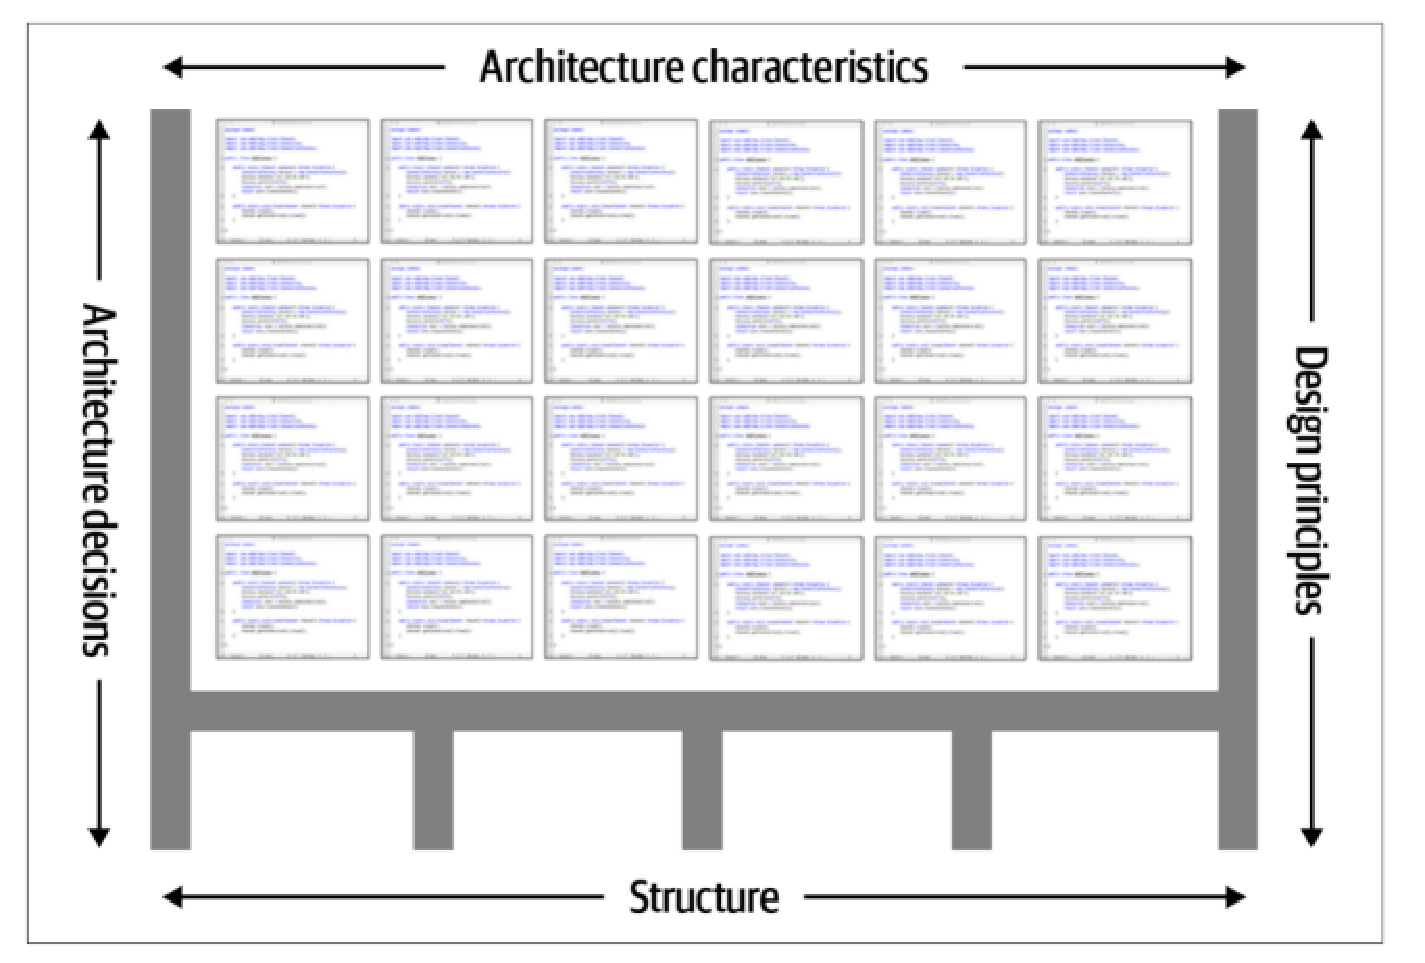
\includegraphics[keepaspectratio=true,scale=0.6]{figuras/richardsAndFord-architectureDefinition.eps}
  \caption{Estrutura básica de um monolítico\label{fig:monolithicStructure} \source{Richards2020:FundamentalsOfSoftwareArchitecture}}
\end{figure}

\begin{description}
    \item [Camada de apresentação] destinada a apresentação dos dados;
    \item [Camada de negócios] destinada a implementação das regras de negócio da aplicação;
    \item [Camada de persistência] destinada a comunicação com o banco de dados;
    \item [Camada de dados] destinada aos armazenamentos dos dados.
\end{description}

\citeonline{StefanTilkov:DontStartWithAMonolith} defende que essa arquitetura é um modelo
essencialmente acoplado, no qual as abstrações que compõe o sistema compartilham de todos os mesmos
recursos da aplicação: bibliotecas, canais de comunicação dentro do próprio processo, modelos de
persistência no banco de dados, etc. A \autoref{fig:monolithicInPractice} exemplifica como mesmo no
modelo modularizado é fácil ultrapassar os limites definidos para cada módulo visto que não há barreiras
técnicas que impeçãm os desenvolvedores de tal. Dessa forma, garantir as características de alta coesão
e baixo acoplamento, tão desejadas na manutenibilidade dos softwares, se torna uma tarefa difícil dependendo
exclusivamente da disciplina dos desenvolvedores \cite{StefanTilkov:DontStartWithAMonolith,MartinFowler:MicroserviceTradeOffs}.

\begin{figure}[h]
  \centering
  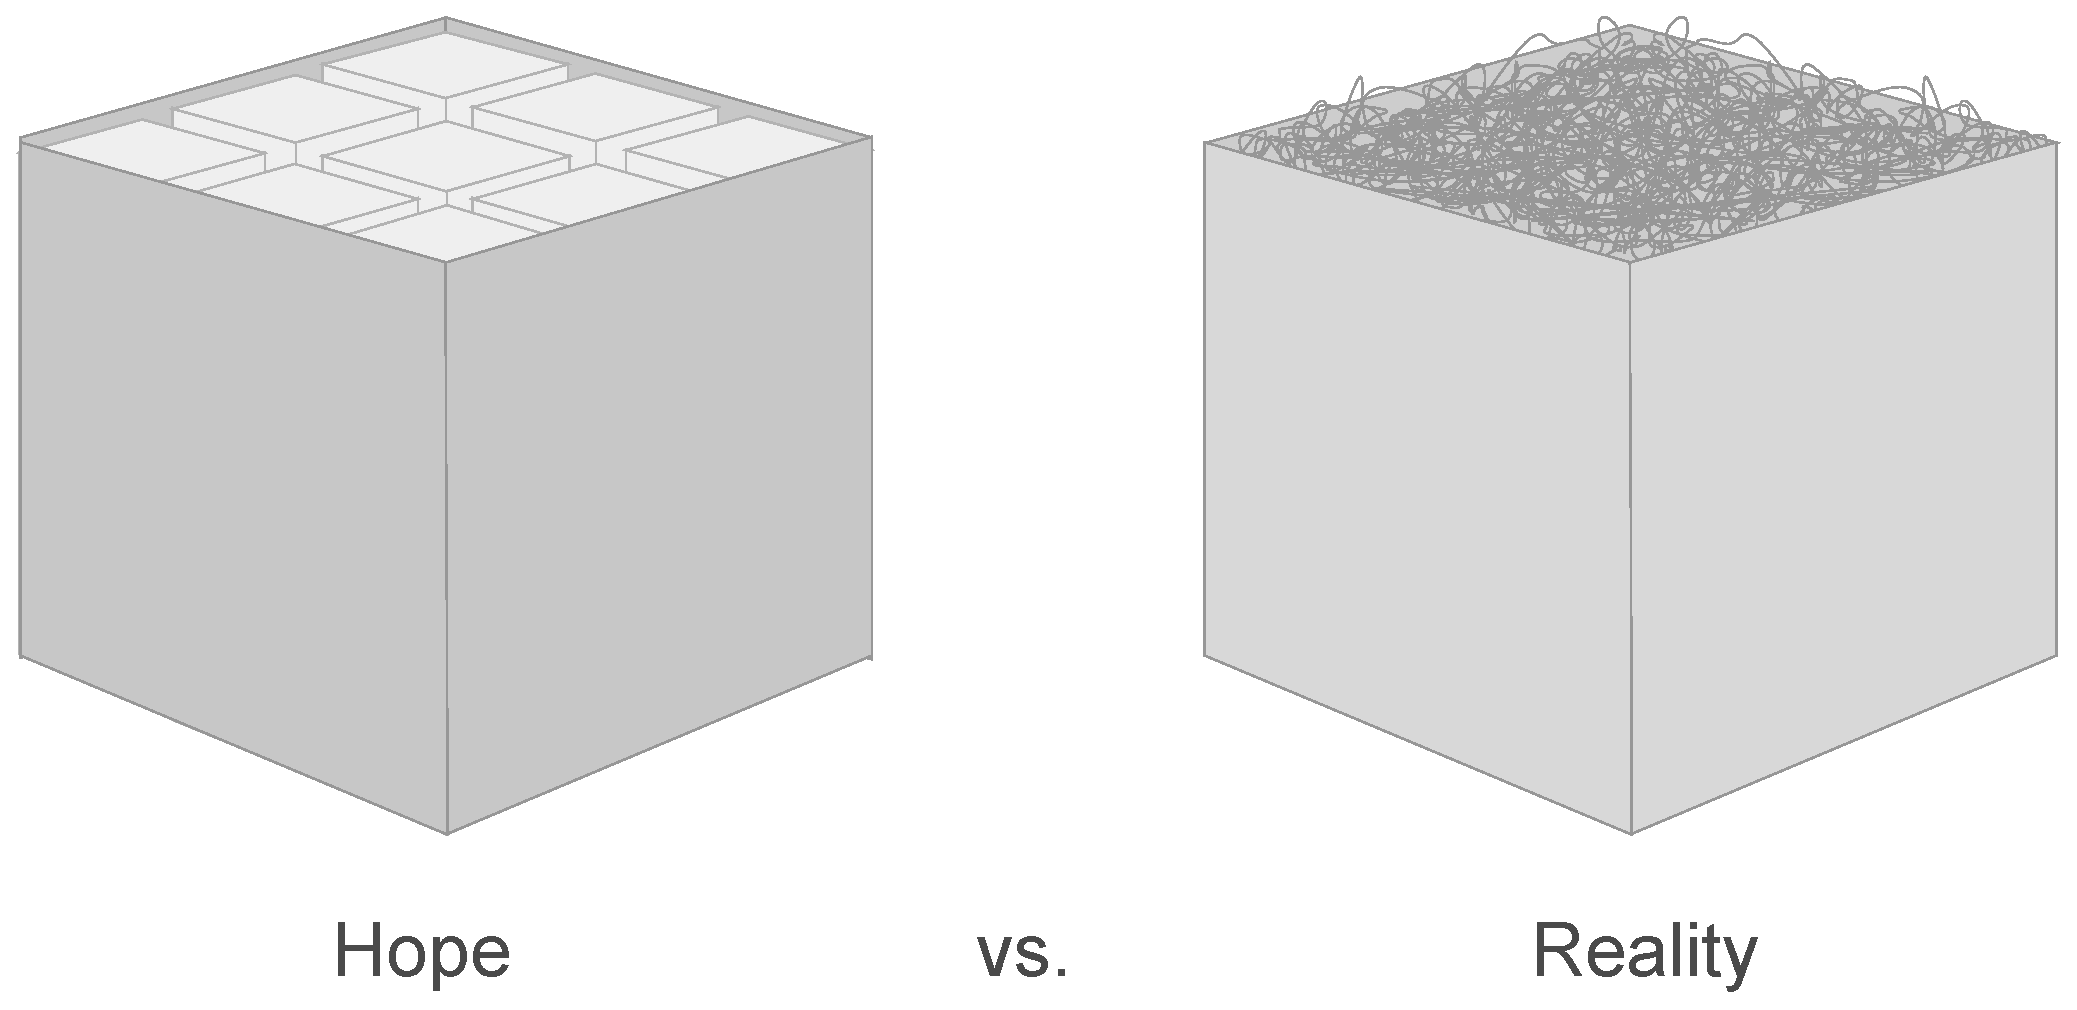
\includegraphics[keepaspectratio=true,scale=0.4]{figuras/monolith-theory-practice.eps}
  \caption{Teoria vs Realidade de um monolítico\label{fig:monolithicInPractice} \source{StefanTilkov:DontStartWithAMonolith}}
\end{figure}

A \autoref{fig:monolithicsharedcomponents} aprofunda ainda mais nesse contexto da arquitetura
monolítica, mostrando a tendência de compartilhar componentes, a exemplo classes de \textit{log},
classes com funções compartilhadas por todo o sistema, etc., transparecendo como a reausabilidade do
código dentro de sistemas monolíticos tende a aumentar o acoplamento entre seus componentes
\cite{Richards2020:FundamentalsOfSoftwareArchitecture}.

\begin{figure}[h]
  \centering
  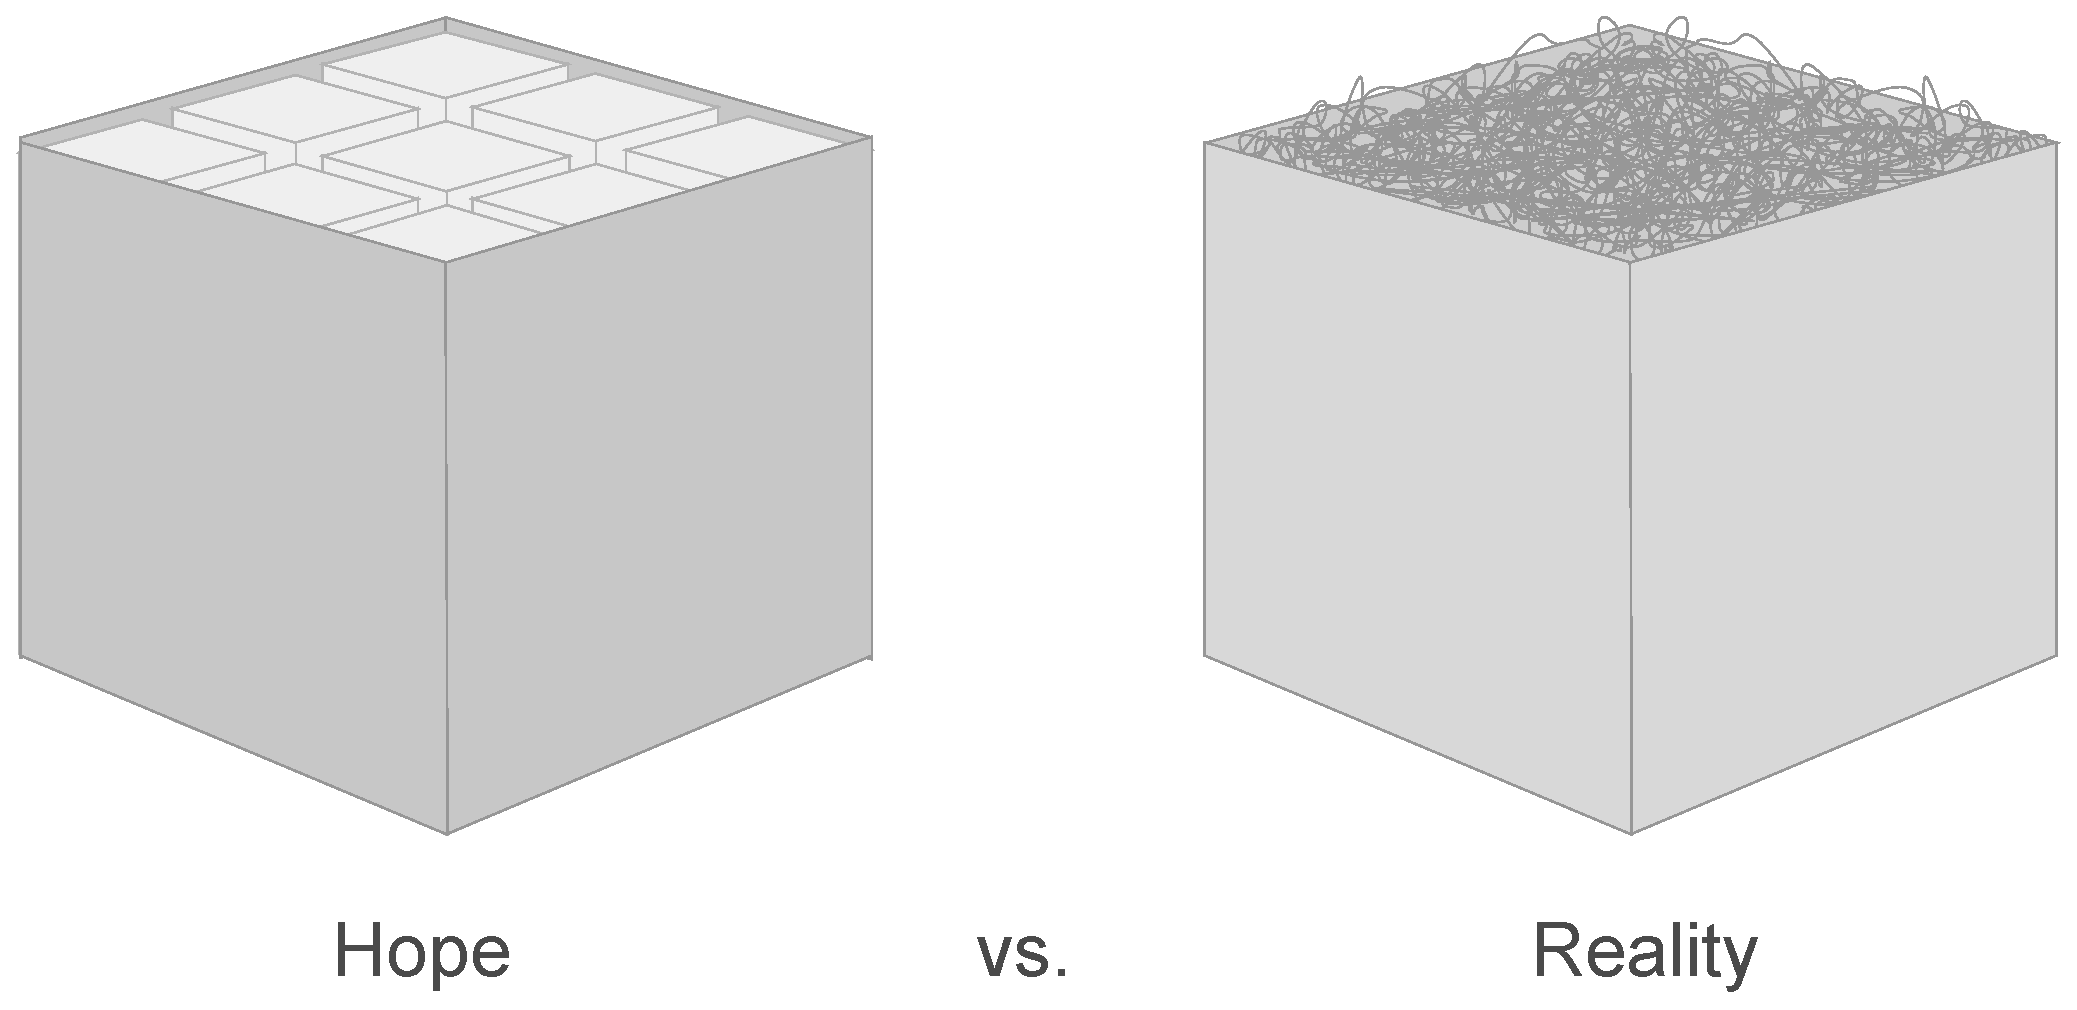
\includegraphics[keepaspectratio=true,scale=0.4]{figuras/monolith-theory-practice.eps}
    \caption{PAGINA 189\label{fig:monolithicsharedcomponents} \source{StefanTilkov:Richards2020:FundamentalsOfSoftwareArchitecture}}
\end{figure}

\section{Microsserviços}

Segundo \citeonline{Richards2020:FundamentalsOfSoftwareArchitecture}, microsserviços é um estilo
arquitetural fortemente inspirado nas ideias de \gls{DDD}, trazendo deste design o conceito de limites
de contexto. Esses limites referem-se a um domínio sob o qual estão entidades e comportamentos que
podemos desacoplar do restante do sistema. Essa abordagem torna os microsserviços pequenos serviços
autônomos que trabalham juntos, em cima de uma base de código coesa e focada em resolver as regras de
negócio dentro do domínio especificado \cite{Newman2015}.

Dessa forma, a aplicação deixa de ser um único processo e passa a ser vários serviços rodando em
processos separados e independentes, os quais se comunicam por meio de algum protocolo \textit{web}
\cite{MartinFowler:Microservices}.

%
% \begin{enumerate}
%     \item{Uso de tecnologias heterogêneas;}
%     \item{Maior resiliência do sistema;}
%     \item{Facilidade em escalar pequenas partes do sistema, ao invés do sistema por
%     completo;}
%     \item{Facilidade e maior estabilidade no processo de \textit{deploy};}
%     \item{Maior produtividade da equipe, uma vez que se passa a adotar equipes
%     menores com bases de código menores;}
%     \item{Reusabilidade dos serviços;}
%     \item{Otimização da substituibilidade: organizações de médio e grande porte costumam
%     possuir sistemas legados, com uma base de código enorme funcionando com tecnologias
%     antigas tanto de software quanto de hardware. A substituição desses códigos é um
%     processo custoso e arriscado. Com serviços pequenos realizar essa substituição
%     se torna um processo mais fácil de gerenciar.}
% \end{enumerate}
%
% Para o desenvolvimento de microsserviços é necessário pensar sobre o que deve ser
% exposto e o que deve ser ocultado. Se houver muito compartilhamento os serviços de
% consumo se acoplam às nossas representações internas, diminuindo a nossa autonomia
% e consequentemente a nossa capacidade de realizar alterações \cite{Newman2015}.

\section{Perspectivas a respeito de cada estilo arquitetural}

Esta seção visa aprofundar no entendimento sobre as vantagens e desafios encontrados na adoção
de cada um dos estilos arquiteturais abordados nesse trabalho. Para tal, será explorado as seguintes
perspectivas com o intuito de compreender como a escolha da arquitetura impacta ou é impactada pelas
mesmas:

\begin{enumerate}
    \item Problemática a ser resolvida;
    \item Recursos necessários
    \item Características arquiteturais;
    \item Manutenibilidade;
    \item Evolucionabilidade.
\end{enumerate}

\subsection{Problemática a ser resolvida}
\label{Perpectivas:Problematica}

Ao iniciar um projeto é comum se ter um baixo domínio sobre o problema a ser resolvido. A exemplo,
as denominadas \textit{startups} estão continuamente surgindo no mercado com o intuito de descobrir
e validar suas ideias. Contextos como este trazem as empresas a necessidade de realizar constantes
alterações de forma extremamente rápida no sistema visando atingir um curto ciclo de
\textit{feedback}.

\citeonline{MartinFowler:MonolithFirst} defende que construir uma versão simplista do seu software é
a melhor forma de descobrir o sistema e validar se ele é realmente útil para os seus usuários.
Assim, ele sugere a estratégia "monolítico primeiro", uma vez que a arquitetura monolítica permite
um desenvolvimento fácil por ser de conhecimento da maioria dos desenvolvedores de software e
apresentar baixa complexidade para a execução de tarefas como \textit{deploy}, confecção de testes
e compartilhamento do código.

\citeonline{MartinFowler:MonolithFirst} e \citeonline{Newman:Greenfield} fortalecem essa visão apontando
que conhecer os limites do seu software é de extrema importância antes de iniciar uma arquitetura de
microsserviços. De forma que os custos e impactos de errar os limites de cada serviço nessa arquitetura
tendem a ser muito maiores do que em um software monolítico mal projetado por não conhecer muito bem o
domínio do problema. 

Um outro ponto a ser considerado na problemática da aplicação refere-se ao tamanho que essa
aplicação terá. \citeonline{Richards2020:FundamentalsOfSoftwareArchitecture} apontam que a arquitetura
monolítica é uma arquitetura de menor custo portanto costuma ser uma boa escolha para sistemas
pequenos.

\subsection{Recursos necessários}

\subsubsection{Recursos financeiros}

De acordo com \citeonline{Richards2020:FundamentalsOfSoftwareArchitecture}, a simplicidade da arquitetura
monolítica reflete em seu baixo custo de desenvolvimento e manutenção. Diferentemente, de uma arquitetura
de microsserviços que exige uma série de fatores: monitoramento, replicação, expertise sobre as
ferramentas, etc., fazendo com o que o custo para desenvolver e manter tal arquitetura seja elevado.
Mediante essa visão, os autores indicam o uso desse modelo para empresas de grande porte,
enquanto que empresas pequenas tendem a lhe dar melhor com monolíticos.

\subsubsection{Recursos humanos}

Na seção \autoref{Perpectivas:Problematica}, nós enfatizamos a importância de conhecer os limites da
sua aplicação antes de optar por uma arquitetura de microsserviços. Isso nos leva a uma outra necessidade desse
estilo arquitetural, referente a relevância de possuir alguém na equipe que detenha esse conhecimento
aprofundado acerca do negócio e da problemática abordada. No texto \textit{Microservices For
Greenfield?}, \citeonline{Newman:Greenfield} relata um projeto no qual eles estavam reimplementando
um sistema que já existia há muitos anos, mas com uma equipe relativamente nova, ou seja, apesar do
domínio de negócio ter sido explorado por um bom tempo, eles não possuíam a expertise necessária
para a construção da aplicação de forma distribuída.

Nesse contexto, \citeonline{Newman:Greenfield} indica a adoção de uma arquitetura monolítica como uma
melhor opção uma vez que, como citado na \autoref{Perpectivas:Problematica}, este estilo arquitetural
é indicado para contextos nos quais não se possui domínio e, para completar, apresenta a vantagem de ser uma
arquitetura familiar para boa parte dos desenvolvedores
\cite{Richards2020:FundamentalsOfSoftwareArchitecture}, dessa forma, ele se diferencia de uma
arquitetura de microsserviços por não precisar de um especialista sobre a tecnologia e sobre o contexto.


\subsubsection{Esforço e tempo inicial}
\label{effortsAndTime}

O tempo de lançamento no mercado costuma ser um fator prioritário para diversas empresas, em geral,
elas desejam lançar o produto no menor tempo possível, seja para validar a ideia, como
vimos na \autoref{Perpectivas:Problematica}, ou por uma questão estratégica de mercado.

Nesse sentido, \citeonline{MartinFowler:MicroservicePremium} aponta que a arquitetura de
microsserviços consegue te entregar uma séries de recompensas (escalabilidade, tolerância a falhas,
etc.) contudo, essas recompensas vêem acompanhada do alto custo que é inerente dos sistemas distribuídos.
Esse modelo arquitetural necessita de \textit{deploy} automatizado, monitoramento, lidar com
eventuais inconsistências dos dados e outros fatores que acabam contribuindo para aumentar o tempo e o esforço
inicial necessário para lançar um produto no mercado. Nas palavras de
\citeonline{Richards2020:FundamentalsOfSoftwareArchitecture}:

\begin{quotation}{Richards2020:FundamentalsOfSoftwareArchitecture}{transleted=true}
    Microsserviços não poderiam existir sem a revolução \textit{DevOps} e a implacável marcha em direção à
    automação de questões operacionais.\footnote{Texto original: \textit{Microservices couldn't exist
    without the DevOps revolution and the relentless march toward automating operational concerns.}}
\end{quotation}

Por outro lado, a simplicidade da arquitetura monolítica permite que funcionalidades cheguem muito
mais rápido no mercado, uma vez que nesse modelo não há tais necessidades e processos como
\textit{deploy} podem ser realizados de maneira operacional. Contudo, vale ressaltar que essa alta
produtividade inicial tende a decrescer com o tempo, a medida que o monolítico vai ganhando mais
funcionalidades e, consequentemente, aumentando a sua complexidade.

\subsection{Características arquiteturais}

\subsubsection{Escalabilidade}

A arquitetura monolítica pode ser escalada horizontalmente utilizando de um \textit{load
balancer}\footnote{\textcolor{red}{DESCREVER}} para executar várias instâncias do sistema
\cite{MartinFowler:Microservices}. Entretanto, a escalabilidade oferecida por essa arquitetura é
bastante limitada. A falta de modularidade exige que toda a aplicação seja replicada ao invés
de replicarmos somente as funções que apresentam maior demanda. Existe a possibilidade de aplicar técnicas
que amenizam esse problema, contudo, isto requer um esforço considerável para adaptar o modelo
arquitetural \cite{Richards2020:FundamentalsOfSoftwareArchitecture}.

No caso dos microsserviços, a escalabilidade é um fator predominante mediante a sua estrutura
altamente desacoplada que favorece a escalabilidade em um nível incremental. Essa característica é
ainda apoiada pelas técnicas modernas de provisionamento de recursos que beneficiam a elasticidade
do estilo arquitetural \cite{Richards2020:FundamentalsOfSoftwareArchitecture}.

\subsubsection{Volume de dados}

\subsubsection{Disponibilidade}

\subsubsection{Tolerância a falhas}

O padrão arquitetural monolítico não suporta tolerância a falhas visto que se algo inesperado
acontece em uma determinada parte do código, como uma leitura de memória inválida, essa falha se
propaga até matar o processo no qual roda todo o código monolítico, indisponibilizando a
aplicação por inteiro, a qual pode levar em média, dependendo do tamanho do monolítico, de de 2 a
15 minutos para ser reinicializada \cite{Richards2020:FundamentalsOfSoftwareArchitecture}.

Do outro lado, os microsserviços naturalmente apresentam aspectos positivos em relação a tolerância
a falhas uma vez que uma falha em um serviço tende a impactar somente uma parte da aplicação.
\citeonline{Richards2020:FundamentalsOfSoftwareArchitecture} fazem uma ressalva que essa tolerância pode
decair se houver muita dependência comunicativa entre os serviços, por isso definir cuidadosamente a
granularidade do serviço é um ponto que deve bem avaliado.

\subsubsection{Confiabilidade}

A arquitetura monolítica quando comparada a uma arquitetura distribuída, como microsserviços, tende
a apresentar maior confiabilidade uma vez que esta não possui os problemas de conexão da rede,
largura de banda e latência que os mesmos apresentam. Contudo, como será abordado na
\autoref{testabilidade}, a testabilidade é um problema desse modelo arquitetural e consequentemente
isso decresce a confiabilidade do sistema \cite{Richards2020:FundamentalsOfSoftwareArchitecture}.

\subsubsection{Performance}

A característica desacoplada dos microsserviços traz consigo um enorme número de requisições
sendo disparadas na rede juntamente com várias camadas adicionais de segurança na comunicação entre
os serviços, o que faz com que o tempo de processamento cresça, tornando este um modelo arquitetural
de baixa performance \cite{Richards2020:FundamentalsOfSoftwareArchitecture}.

A característica simplista dos monolíticos também não contribui nesse quesito. Segundo
\citeonline{Richards2020:FundamentalsOfSoftwareArchitecture}, a arquitetura monolítica não é por si
mesma uma arquitetura de alta performance, exigindo esforço dos engenheiros para proporcionar
tal fator para a aplicação por meio de desenvolvimento paralelo, \textit{multithreading}, etc.

\subsection{Manutenibilidade}

\subsubsection{\textit{Deploy}}
Na \autoref{monolithics} foi apresentado como monolíticos são em sua essência uma unidade de
\textit{deploy}. No início do projeto, esta característica contribui com a simplicidade e a
velocidade em lançar o sistema, como relatado na \autoref{effortsAndTime}. Porém, a medida que a
base de código do monolítico cresce, compilar e implantar toda a base de código a fim de
disponibilizar uma alteração tende a se tornar um processo árduo, fazendo com que seja difícil e
demorado disponibilizar as mudanças realizadas no sistema \cite{MartinFowler:Microservices}. Para
completar o quadro, o \textit{deploy} de uma versão da aplicação monolítica com um \textit{bug},
por exemplo, acresce os riscos dessa alteração atingir o banco de dados ou alguma outra parte do
sistema, torando a reversão do impacto do processo de implantação mais difícil
\cite{Richards2020:FundamentalsOfSoftwareArchitecture}.

Os microsserviços apresentam o caminho inverso: inicialmente eles exigem mais esforços para
implantar, visto que é necessário automatizar todas as partes do fluxo de implantação, todavia, uma
vez que os processos estão automatizados, disponibilizar mudanças no sistema se torna uma tarefa
fácil e rápida. Essa abordagem se caracteriza por somente uma parte do código ser enviada para
produção, minimizando os impactos que possam ocorrer ao disponibilizar a funcionalidade.

\subsubsection{Testabilidade}
\label{testabilidade}

A testabilidade de uma arquitetura monolítica é apontada por \citeonline{Richards2020:FundamentalsOfSoftwareArchitecture}
como um ponto fraco nesse estilo arquitetural. Os autores defendem que este é um aspecto que decresce a
medida que a complexidade do sistema aumenta e, dessa forma, desenvolvedores ao fazerem uma pequena
modificação tendem a não executar toda a \textit{suite} de testes devido ao alto custo de tempo para
tal.

Já para uma arquitetura de microsserviços, eles consideram a testabilidade um ponto positivo, visto que
cada serviço pode ser testado facilmente dentro do seu domínio. \citeonline{MartinFowler:Microservices}
ressaltam que a base desse modelo arquitetural são os limites de domínio de cada serviço, e
para tal é importante coordenar qualquer mudança nas interfaces de comunicação adicionando camadas
extras de compatibilidade de versões, o que acaba tornando o processo de testes mais difícil.

\subsubsection{\textit{Debugger}}
\subsubsection{Curva de aprendizado}
\subsubsection{Comunicação}

\begin{quotation}{Conway}{transleted=true}
    Qualquer organização que projeta um sistema (definido de forma mais ampla aqui do que apenas sistemas de informação)
    produzirá inevitavelmente um projeto cuja estrutura é uma cópia da estrutura de comunicação da
    organização.\footnote{Texto original: \textit{Any organization that designs a system (defined more broadly
    here than just information systems) will inevitably produce a design whose structure is a copy
    of the organization's communication structure.}}
\end{quotation}

\citeonline{MartinFowler:Microservices} faz uma menção a Lei de Conway apresentada acima,
exemplificando-a na \autoref{fig:conwayMonolithic} como essa arquitetura em camadas reflete a
organização das empresas. Eles apontam que essa estrutura deixa a comunicação dentro do projeto mais
lenta, de forma que mudanças simples no sistema podem demorar bastante devido a dependência de uma
equipe externa.

\begin{figure}[h]
  \centering
  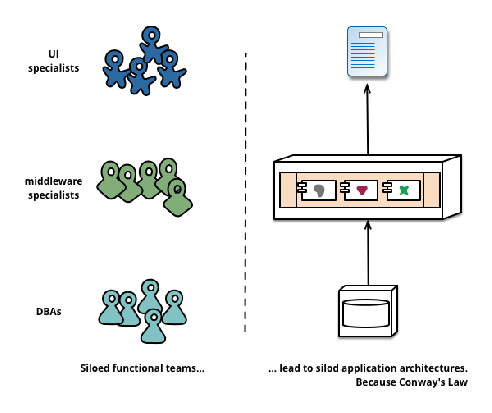
\includegraphics[keepaspectratio=true,scale=1]{figuras/conwayMonolithic.eps}
  \caption{Lei de Conway aplicada a uma arquitetura em camadas\label{fig:conwayMonolithic} \source{MartinFowler:Microservices}}
\end{figure}

Quando olhamos para essa estrutura organizacional dentro da arquitetura de microsserviços,
\autoref{fig:conwayMicroservices}, a essência desta arquitetura de ser particionada por domínio
do negócio e não por suas características técnicas é refletida gerando times multifuncionais, de
forma que a equipe possua toda a gama de habilidades necessárias \cite{MartinFowler:Microservices}.

\begin{figure}[h]
  \centering
  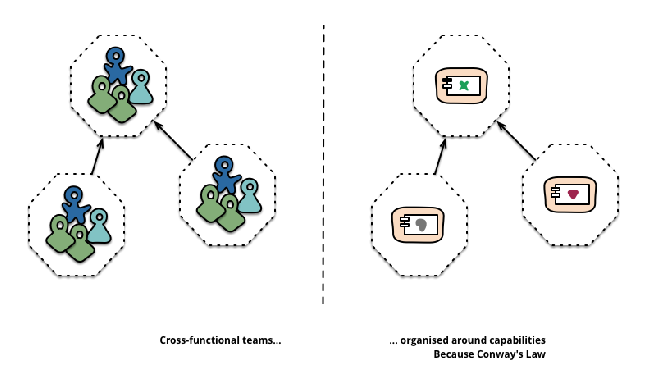
\includegraphics[keepaspectratio=true,scale=1]{figuras/conwayMicroservices.eps}
  \caption{Lei de Conway aplicada a uma arquitetura de microsserviços\label{fig:conwayMicroservices} \source{MartinFowler:Microservices}}
\end{figure}

\subsection{Evolucionabilidade}

\subsubsection{Heterogeneidade das tecnologias}

Tradicionalmente, as empresas padronizam a \textit{stack} de tecnologias com a qual trabalham. Na
arquitetura monolítica esse fator acaba se tornando algo enraizado no sistema devido a sua
característica inerente de ser uma arquitetura acoplada, fazendo com que a adoção de tecnologias
diferentes para cada problema, ou mesmo a migração do sistema para uma tecnologia mais atual seja um
processo bastante árduo.

Os microsserviços já apresentam a característica oposta de serem em sua essência altamente
desacoplados. Isso permite aos engenheiros de software escolherem a melhor tecnologia para escalar a
solução de acordo com problema abordado \cite{Richards2020:FundamentalsOfSoftwareArchitecture}.

\subsubsection{Complexidade}


